[introduction/in-dabc-design.tex]
\section{Design}
\subsection{Task layout}
\begin{figure}[htb]
\centering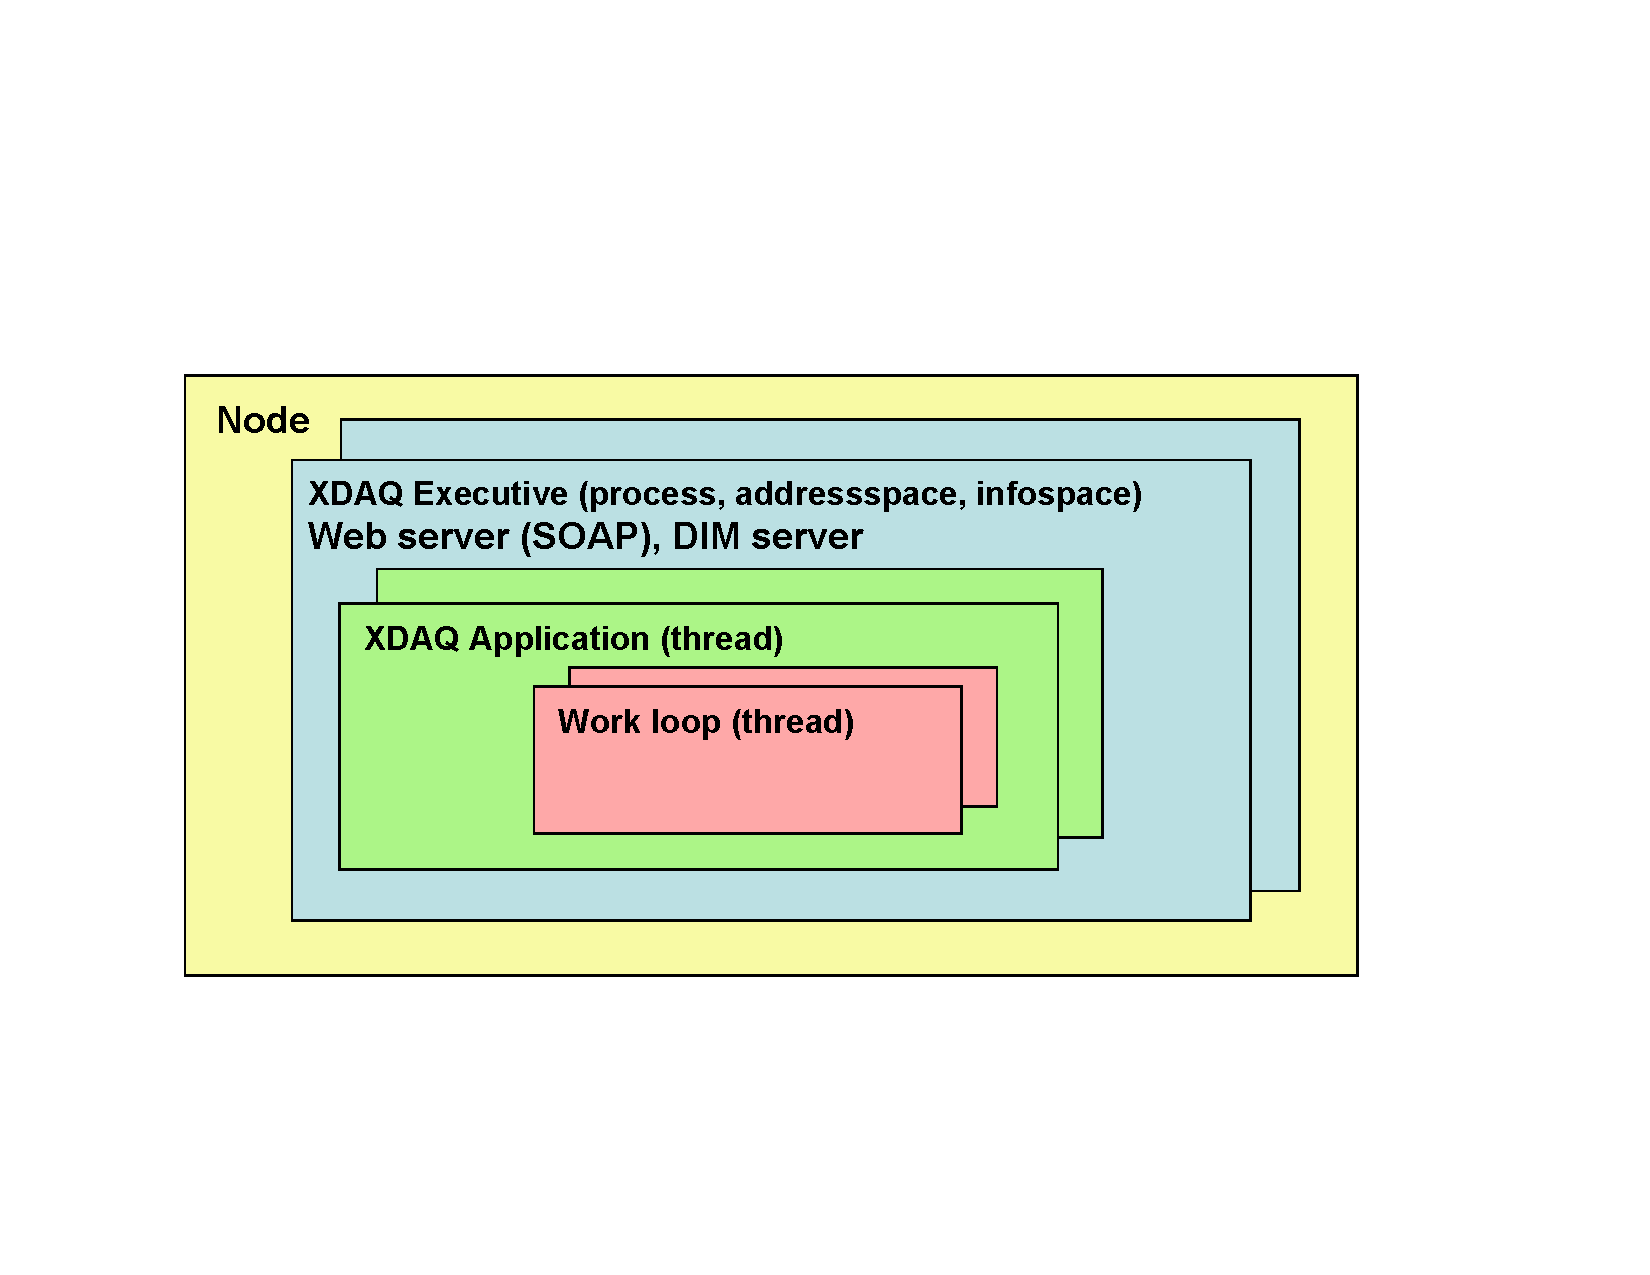
\includegraphics[width=.8\textwidth] {dabc_sw-over_3}
\caption{\xdaq~ entities} \label{fig:dabc_sw-over_3}
\end{figure}
Figure \ref{fig:dabc_sw-over_3} shows the task layout of \xdaq~.
On each node there is at least one executive which controls
the \xdaq~ applications. The applications run in threads
thus being scheduled and sharing memory. Applications also may start and
control threads (work loops).\\
The executive also is the communication stub through the Web interface or the
DIM gateway. The executive addressspace is the scope of the infospace. The
infospace provides mechanisms to access parameters across applications
and subscribe for parameter changes. The DIM gateway subscribes for
parameters in the infospace and serves them to DIM clients.\\
Figure \ref{fig:dabc_sw-over_4}, page \pageref{fig:dabc_sw-over_4} shows the data flow. 
There are two main
\xdaq~ executives. One runs the applications for the data input from the
front-end systems, the event building scheduler and the network senders.
The second one runs the event receiver applications for event tagging,
event building and event senders.
\clearpage
\subsection{MBS data input}
A \dabc~ input channel can connect to an \mbs~ transport and read LMD buffers.
The \mbs~ runs in a special \dabc-mode without event spanning over buffers.
Because buffers now can have any size, one buffer per stream can be configured
to avoid event spanning.

\subsubsection{Communication protocol}
\begin{compactenum}
\item The \dabc~ input channel connects to the \mbs~ transport.
\item An acknowledge message of 4 longwords is returned (endian=1, size, buffers, streams).
For transport that means that \dabc~ needs a buffer of size x buffers bytes to store all
events of a stream completely (no fragments).
\item Start reading buffers. When the reading is slower than the \mbs~ can send,
the \mbs~ blocks!\\
\mbs~ transport sends buffers.
\item Close connection.
\end{compactenum}


\subsubsection{MBS control}
The remote \mbs~ system can be controlled completely by \dabc.
\mbs~ runs now DIM servers for monitoring and controls.
The \mbs~ is started by remote shell commands and controlled by
sending commands to DIM server. The controlling process as a DIM client
registers the \mbs~ status information for monitoring.
